\documentclass[10pt]{beamer}

%\usetheme{metropolis}
\usepackage{appendixnumberbeamer}

\usepackage{pgfplots}
\usepgfplotslibrary{dateplot}

\usepackage{xspace, amsfonts}
\newcommand{\themename}{\textbf{\textsc{metropolis}}\xspace}

\title{Experimental Evaluation of Control Policies for \\Segway Robot in Dynamic Environments }
\author{Ian~Buckley, Niharika~Arora, Varun~Murali}
\date{26 April 2015}
\institute{ECE 6552: Nonlinear System Project}
% \titlegraphic{\hfill\includegraphics[height=1.5cm]{logo.pdf}}

\begin{document}

\maketitle
\section{Motivation}
\begin{frame}{Motivation}
\begin{itemize}
\item<1-> Navigation is a fundamental objective in mobile robotics
\item<2-> Deliberative path planning suffers from unexpected conditions (i.e. Probabilistic Roadmaps \cite{kavraki1996}) 
\item<3-> Reactive methods suffer from local minima (i.e. Potential Fields \cite{khatib1985})
\item<4-> A hybrid approach applies the benefits and mitigates the shortcomings of both
\item<5-> A nonlinear navigation control protocol can achieve navigational objectives while reacting to unexpected obstacles 
\end{itemize}
\end{frame}

\section{System Description}
\begin{frame}{Robotic Platform}
\begin{figure}
    \centering
    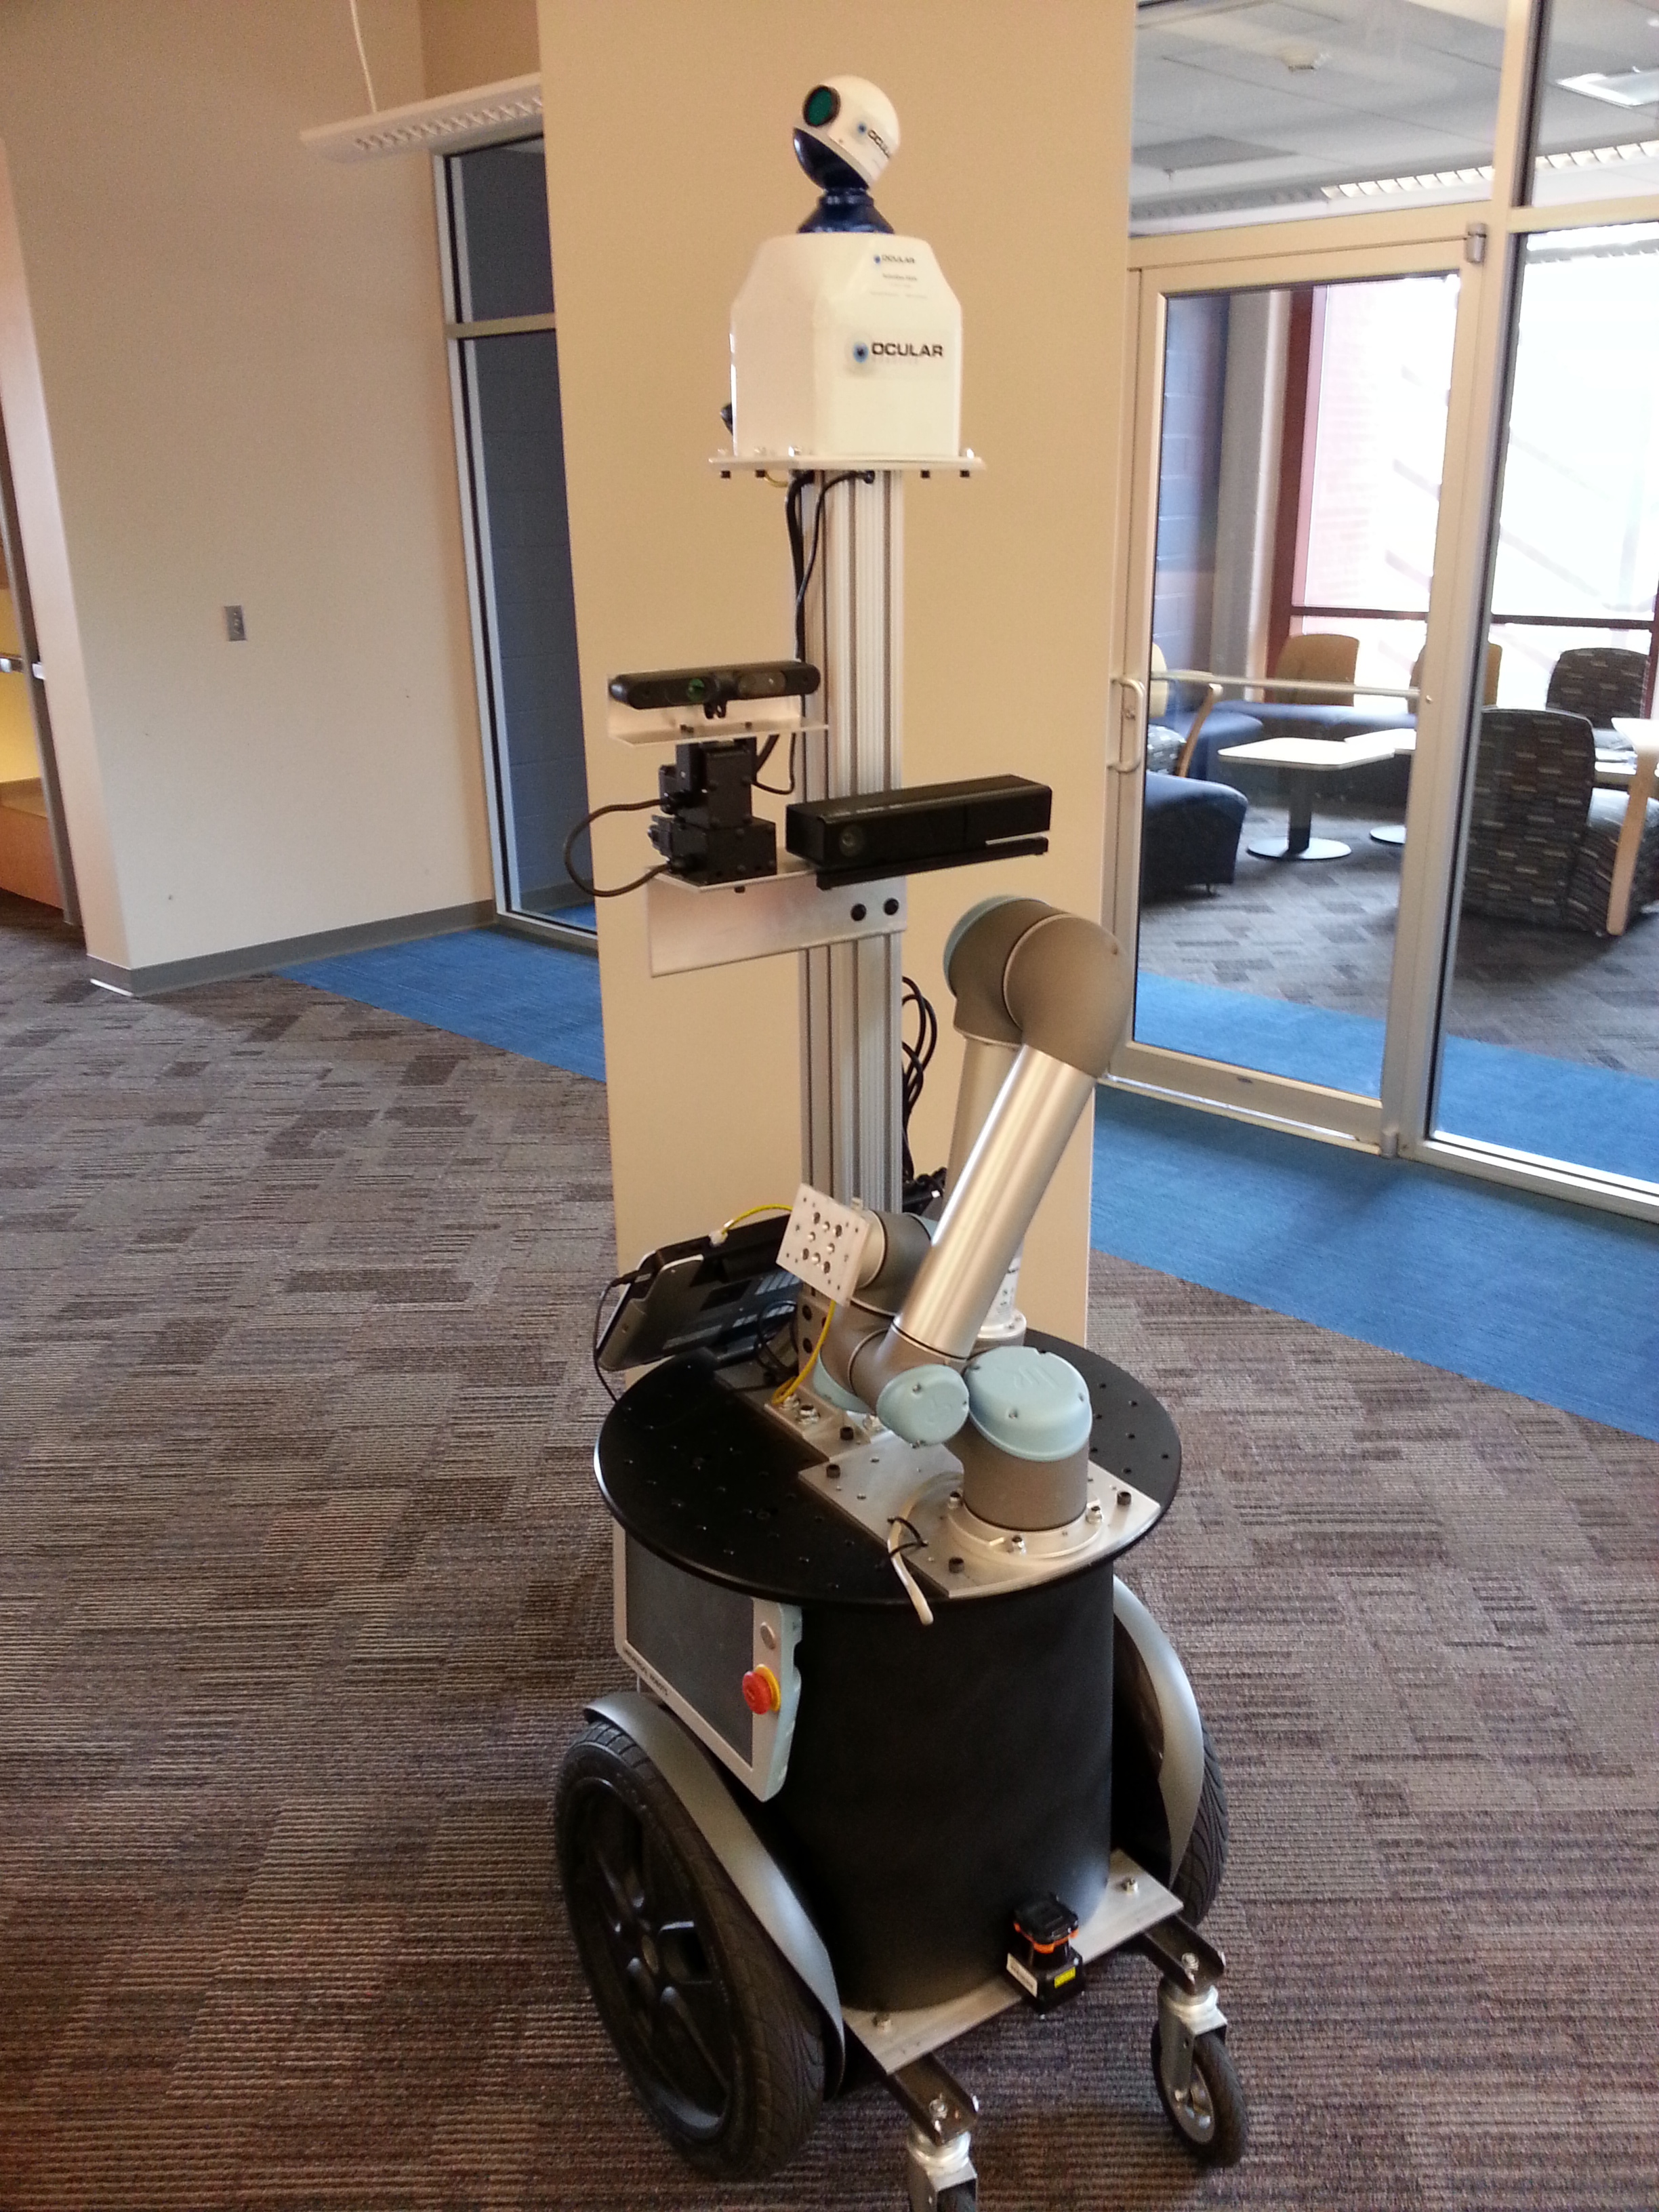
\includegraphics[width = 4cm, scale=0.2]{jeeves2_0.jpg}
    \caption{Jeeves - A modified Segway based robot mounted with a Primesense, Microsfot Kinect, Roboteye RE05, Hokuyo LTM-30x laser and the UR5. Currently modified to include the casters for static stability
    \label{fig:jeeves}}
\end{figure}
\end{frame}

\begin{frame}{Unicycle Dynamics}
\begin{columns}
\column{0.4\linewidth}
\begin{equation}
\left(
\begin{matrix}
\dot{r}\\
\dot{\theta}\\
\end{matrix}
\right)
=
\left(
\begin{matrix}
- v \text{ cos}(\delta)\\
\frac{v}{r} \text{ sin}(\delta)\\
\end{matrix}
\right)
\end{equation}
\begin{equation}
\dot{\delta}=\frac{v}{r} \text{ sin}(\delta)+\omega
\end{equation}
\column{0.6\linewidth}
\begin{figure}[h!]
\begin{center}
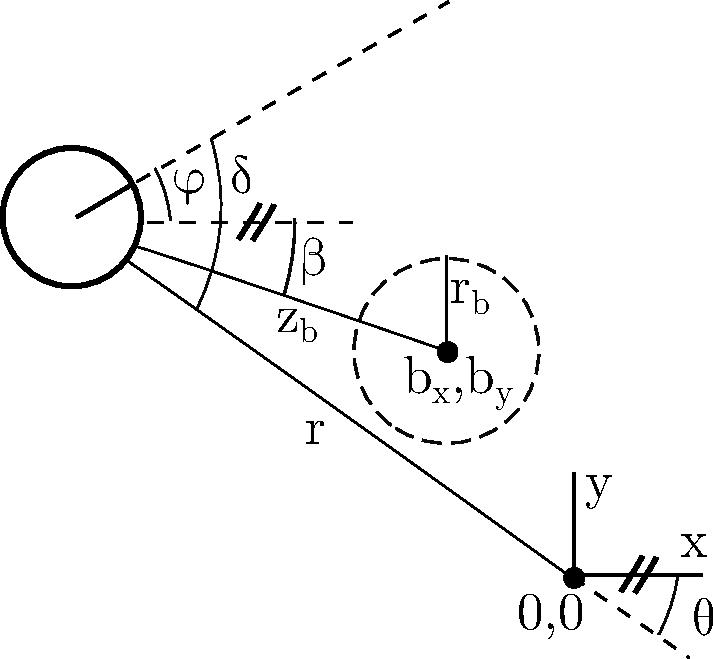
\includegraphics[scale=0.45]{obs.pdf} 
\caption{Egocentric Polar Unicycle Dynamics with Obstacle\label{fig:obs}} 
\end{center}
\end{figure}
\end{columns}
\end{frame}

\section{Approach}
\begin{frame}{Objectives}

\textbf{Soft Constraints}
\begin{itemize}
\item Navigate to target location\\
\item Drive the state of the robot to zero (e.g. $\dot{x}=(\dot{r},\dot{\theta},\dot{delta})^T \to 0$)\\ 
\end{itemize}

\textbf{Hard Constraints}
\begin{itemize}
\item Avoid obstacles\\ 
\item The distance to the obstacle must not exceed a minimum distance (e.g. $z_b>z_{safe}$)\\
\end{itemize}

\textbf{System Constraints}
\begin{itemize}
\item Inputs should not exceed threshold values\\ 
\item $0<v<v_{max}$ and $0<\omega<\omega_{max}$\\
\end{itemize}
\end{frame}

\begin{frame}{Approach Overview}
A \alert{switched mode} \emph{quadratic programming controller} that \textbf{simultaneously} satisfies the soft constraints, hard constraints, and system constraints was designed.
\end{frame}

\begin{frame}{Soft Constraints as CLFs}
To establish soft constraints as CFLs:
\begin{enumerate}
\item<1-> Design a steering control that drives the state to zero \cite{park2011}\\
\item<2-> Demonstrate that the steering control satisfies the control Lyapunov function\\
\item<3-> Design a second steering control that drives the state \textit{away} from zero\\
\end{enumerate}
\end{frame}

\begin{frame}{Soft Constraints as CLFs}
1. \textbf{Design a steering control that drives the state to zero}
%\item Demonstrate that the steering control satisfies the control Lyapunov function\\
%\item Design a second steering control that drives the state \textit{away} from zero\\
$$z_1 = \delta - \text{arctan}(-k_1\theta)$$\pause
$$\dot{z_1}=\left( 1+\frac{k_1}{1+(k_1\theta)^2}\right) \frac{v}{r}\text{ sin}(z_1+\text{ arctan}(-k_1\theta))+\omega$$\pause


Feedback linearization of this objective by choosing the angular velocity: $$\omega = -\frac{v}{r}\left[ k_2 z_1+\left( 1 + \frac{k_1}{1+(k_1\theta)^2} \right) \text{sin}(z_1+\text{ arctan}(-k_1\theta))\right]$$\pause
$$ \dot{z_1}=-k_2\frac{v}{r}z_1 $$\begin{center}
\textit{$\implies$ Stabilization of the steering objective}\end{center}
\end{frame}

\begin{frame}{Soft Constraints as CLFs}
2. \textbf{Demonstrate that the steering control satisfies the control Lyapunov function}
%\item Design a second steering control that drives the state \textit{away} from zero\\
$$\delta=\text{arctan}(-k_1\theta)$$\pause
$$V=\frac{1}{2}(r^2+\theta^2)$$\pause
$$\dot{V}=-r v \text{ cos}(\delta) + \theta v \text{ sin}(\delta)$$\pause
$$\dot{V}=-r v \text{ cos}(\text{arctan}(-k_1\theta)) + \theta v \text{ sin}(\text{arctan}(-k_1\theta))$$\pause
$$\dot{V}<0$$\begin{center}
\textit{$\implies$ Stabilization of the state to zero}\end{center}
\end{frame}

\begin{frame}{Soft Constraints as CLFs}
3. \textbf{Design a second steering control that drives the state \textit{away} from zero}
$$z_2 = \delta - \text{arctan}(-k_1\beta)$$\pause

\begin{center}
Similar to $z_1$... \pause
\end{center}

$$ \dot{z_2}=-k_2\frac{v}{r}z_2 $$
\begin{center}\textit{$\implies$ Stabilization of the second steering objective}\end{center}\pause

$$\dot{V}=-r v \text{ cos}(\text{arctan}(k_1\beta)) + \theta v \text{ sin}(\text{arctan}(-k_1\beta))$$\pause
$$\dot{V}\nleq 0$$\begin{center}
\textit{$\implies$ The second steering control drives the state \alert{away} from zero}\end{center}
\end{frame}

\begin{frame}{Hard Constraint as ZBF \cite{amesACC},\cite{ames2015robust},\cite{ames2014esclf}}
$$\dot{h}(x)<=\gamma h(x)$$\pause
\begin{align*}
C &= {x \in \mathbb{R}^3 | z_b\geq z_{safe}}\\
\partial C &= {x \in \mathbb{R}^3 | z_b=z_{safe}}\\
\text{Int}(C) &= {x \in \mathbb{R}^3 | z_b > z_{safe}}
\end{align*}\pause
$$h(x)=\sqrt{(-v\text{ cos}(\theta)-b_x)^2+(v\text{ sin}(\theta)-b_y)^2}$$\pause
$$\dot{h}(x)=$$

\end{frame}

\begin{frame}{Switched Mode QP Controller}

\end{frame}

\section{Results}
\begin{frame}{Simulation Results}
needs octo plots!
\end{frame}

\begin{frame}{Experimental Results}
needs robots!
\end{frame}

\section{Conclusions}
\begin{frame}{}

\end{frame}

\begin{frame}[allowframebreaks]{References}
\footnotesize
\bibliographystyle{IEEEtran}
\bibliography{IEEEabrv,bibi}
\end{frame}

\begin{frame}[standout]
Questions?
\end{frame}

\end{document}